\chapter{Forecasting epidemic surges of competing pathogen variants}
\graphicspath{{figures/ch_5/}}
\label{ch:content_3}

\section{Introduction}
\label{ch_5:sec:intro}

\begin{itemize}
    \item Forecasting in Epidemic modeling is important.
    \item A lot of forecasting methods have been tried recently.
    \item COVID-19 saw changing dynamics due to new variants
    \item When new variants arise, they can lead to waves, either due to increased transmissibility or immune escape
    \item We would like to incorporate this data into our models in a simple, but flexible way.
    \item Multi-strain models have been proposed, but are rarely (never?) fit to data.
    \item We base our forecasting on mechanistic modeling.
    \item We assess our models in a simulation study with different takeover speeds
    \item We apply to real data from Orange County, CA and the entire state of CA.
    \item We show our method is superior at forecasting and esp at forecasting peak timing of hosp (something healthcare people care a lot about) compared to a typical semi-parametric model.
\end{itemize}

\section{Methods}
\label{ch_5:sec:methods}

\subsection{Data}
\label{ch_5:subsec:data}

We work with time series of daily numbers of cases, infected hospital occupants, infected ICU occupants, deaths due to the infection, genetic sequences from a novel variant, and genetic sequences from other variants.
These time series need not be observed at the same temporal resolution, but, for clear exposition in this section, we assume they are each reported at times \( t_1, \ldots, t_L \).
We denote the vector of cases, \( \bW = \left( W_1, \ldots, W_L \right) \); infected hospital occupants, \( \bX = \left( X_1, \ldots, X_L \right) \); infected ICU occupants, \( \bY = \left( Y_1, \ldots, Y_L \right) \); deaths due to the infection, \( \bZ = \left( Z_1, \ldots, Z_L \right) \); genetic sequences from the novel variant, \( \bV^N =  \left( V^N_1, \ldots, V^N_L \right)\); genetic sequences from other variants, \( \bV^O =  \left( V^O_1, \ldots, V^O_L \right)\). In each vector, the subscript indicates that the observation is made at the corresponding time, \( t_1, \ldots, t_L \).
We work up to a surveillance model for these time series by first describing a transmission model for the underlying population dynamics.

\subsection{Transmission model}
\label{ch_5:subsec:transmission}

We model latent incidence and prevalence trajectories by dividing the population of interest into seven compartments: susceptible individuals \( (S) \), infected, but not yet infectious, individuals \( (E) \), infectious individuals \( (I) \), individuals hospitalized with infection \( (H) \), individuals in the ICU with infection \( (U) \),  recovered individuals \( (R) \), and individuals who died due to infection \( (D) \).
The potential progression of an individual through these states is presented in Figure~\ref{ch_5:fig:model_diagram}.
\begin{figure}
    \centering
% https://q.uiver.app/?q=WzAsNyxbMCwyLCJTIl0sWzEsMiwiRSJdLFsyLDIsIkkiXSxbNCwyLCJSIl0sWzQsMCwiRCJdLFsyLDEsIkgiXSxbMiwwLCJJQ1UiXSxbMCwxXSxbMSwyXSxbMiwzXSxbMywwLCIiLDAseyJjdXJ2ZSI6LTV9XSxbNSwzXSxbNiwzXSxbNiw0XSxbNSw2XSxbMiw1XV0=
\begin{tikzcd}[sep=scriptsize]
	&& U && D \\
	&& H \\
	S & E & I && R
	\arrow[from=3-1, to=3-2]
	\arrow[from=3-2, to=3-3]
	\arrow[from=3-3, to=3-5]
	\arrow[curve={height=-30pt}, from=3-5, to=3-1]
	\arrow[from=2-3, to=3-5]
	\arrow[from=1-3, to=3-5]
	\arrow[from=1-3, to=1-5]
	\arrow[from=2-3, to=1-3]
	\arrow[from=3-3, to=2-3]
\end{tikzcd}
    \caption[State transition diagram.]{Model diagram for potential progression between infection states.
    Model compartments are susceptible individuals \( (S) \), infected, but not yet infectious, individuals \( (E) \), infectious individuals \( (I) \), individuals hospitalized with infection \( (H) \), individuals in the ICU with infection \( (U) \),  recovered individuals \( (R) \), and individuals who died due to infection \( (D) \).}
    \label{ch_5:fig:model_diagram}
\end{figure}
We model the time-evolution of the proportions of individuals occupying these compartments with a set of deterministic ordinary differential equations (ODEs).
For simplicity, we assume a homogeneously mixing population of fixed size \( N \).
Let \( \bA(t) = \left(S(t) \right.\), \( E(t) \), \( I(t) \), \( H(t) \), \( U(t) \), \( R(t) \), \( \left. D(t) \right)^T \) denote the population proportion in each compartment at time \( t \).
We normalize \( \bA(t_0) \) so that \( \bA(t_0)^T\boldsymbol{1} = 1\), where \( \boldsymbol{1} = (1, 1, 1, 1, 1, 1, 1)^T \).
Because we fit this model to incidence data, it is convenient to also keep track of the cumulative proportion of the population that experiences transitions between compartments from \( t_0 \) to \( t \): \( \bN(t) = \left(N_{SE}(t) \right. \), \( N_{EI}(t) \), \( N_{IH}(t) \), \( N_{HU}(t) \), \( N_{UD}(t) \), \( N_{IR}(t) \), \( N_{HR}(t) \), \( N_{UR}(t) \), \( \left. N_{RS}(t) \right)^T\).
To describe mathematically how vectors $\bA(t)$ and $\bN(t)$ change through time, we first define rates of transitions between compartments, with possible transitions corresponding to the arrows in Figure~\ref{ch_5:fig:model_diagram}:

\begin{equation}
\begin{aligned}
\lambda_{SE}(S, I)  =&  \frac{\beta}{N} S I   \\
\lambda_{EI}(E)  =& \gamma E    \\
\lambda_{IH}(I)  =& \nu \tau I   \\
\lambda_{HU}(H)  =& \eta  \upsilon H   \\
\lambda_{UD}(U)  =& \omega \chi U \\
\end{aligned}
\qquad \quad \quad
\begin{aligned}
\lambda_{IR}(I)  =& \nu \left(1 - \tau \right) I   \\
\lambda_{HR}(H)  =& \eta \left(1 - \upsilon \right) H \\
\lambda_{UR}(U)  =& \omega \left( 1 - \chi \right) U    \\
\lambda_{RS}(R)  =& \kappa R
\end{aligned}
\label{ch_5:eqn:transition_rates}
\end{equation}

where \( \beta \) is the transmission rate, \( N \) is the constant population size, \( 1 / \gamma  \) is the mean latent period duration, \( 1 / \nu \) is the mean infectious period duration, \( 1 / \eta \) is the mean hospitalization duration, \( 1 / \omega \) is the mean ICU stay duration, \( 1 / \kappa \) is the mean immune duration, \( \tau \) is the infection-hospitalization ratio, \( \upsilon \) is the hospitalization-ICU admission ratio, and \( \chi \) is the ICU-fatality ratio.
In some cases, we can allow certain parameters to vary in time to capture changing dynamics without the needing for additional compartments in the model.
These changing dynamics could be due to policy or behavioral changes, or the presence of a new variant with increased transmissibility or immune escape.
In particular, in the models we consider in our simulation study and application, we replace \( \beta \) and \( \kappa \) with time-varying versions, \( \beta(t) \), and \( \kappa(t) \).
We discuss the details of this implementation in Section~\ref{ch_5:subsec:bayesian}.

Using the transition rates in \eqref{ch_5:eqn:transition_rates}, we define the ODEs in the model:

\begin{equation}
\begin{aligned}
\deriv{S}{t}    =&  \lambda_{RS}(R) - \lambda_{SE}(S, I) \\
\deriv{E}{t}    =&  \lambda_{SE}(S, I) - \lambda_{EI}(E)    \\
\deriv{I}{t}    =&  \lambda_{EI}(E) - \left( \lambda_{IH}(I) + \lambda_{IR}(I) \right)\\
\deriv{H}{t}    =&  \lambda_{IH}(I) - \left( \lambda_{HU}(H) +  \lambda_{HR}(H) \right)\\
\deriv{U}{t}    =&  \lambda_{HU}(H) - \left( \lambda_{UD}(U) + \lambda_{UR}(U) \right)\\
\deriv{D}{t}    =&  \lambda_{UD}(U) \\
\deriv{R}{t}    =&  \left( \lambda_{IR}(I) + \lambda_{HR}(H) + \lambda_{UR}(U) \right) - \lambda_{RS}(R)    \\
\end{aligned}
\qquad
\begin{aligned}
\deriv{N_{SE}}{t}  =&  \lambda_{SE}(S, I) \\
\deriv{N_{EI}}{t}  =&  \lambda_{EI}(E) \\
\deriv{N_{IH}}{t}  =&  \lambda_{IH}(I) \\
\deriv{N_{HU}}{t}  =&  \lambda_{HU}(H) \\
\deriv{N_{UD}}{t}  =&  \lambda_{UD}(U) \\
\deriv{N_{IR}}{t}  =&  \lambda_{IR}(I) \\
\deriv{N_{HR}}{t}  =&  \lambda_{HR}(H) \\
\deriv{N_{UR}}{t}  =&  \lambda_{UR}(U) \\
\deriv{N_{RS}}{t}  =&  \lambda_{RS}(R)
\end{aligned}
\label{ch_5:eqn:ODEs}
\end{equation}
subject to initial conditions \( \bA(t_0) = \left( S_0, E_0, I_0, H_0, U_0, D_0, R_0 \right) \).
Because the total population size is fixed at size \( N \), and we take \( H_0 \) , \( U_0 \), and \( D_0 \) to match the reported values of the hospitalizations, ICU occupancy, and deaths in the data at \( t_0 \), we are left with \( E_0 \), \( I_0 \), and \( R_0 \) as free parameters (because \( S_0 = N - \left( E_0 + I_0 + H_0 + U_0 + D_0 + R_0 \right) \).
The equations in \eqref{ch_5:eqn:ODEs} are redundant, but tracking both the prevalence (left column) and the cumulative incidence (right column) are useful for linking the transmission model to data via a surveillance model.

\subsection{Surveillance model}
\label{ch_5:subsec:surveillance}

We fit the transmission model to six time series: number of new cases \( \left( \bW \right) \),  number of infected hospital occupants \( \left( \bX \right) \), number of infected ICU occupants \( \left( \bY \right) \), number of new deaths due to the infection \( \left( \bZ \right) \), number of  genetic sequences from the novel variant \( \left( \bV^N \right) \), and number of genetic sequences from other variants \( \left( \bV^O \right) \) observed at time points \( t_1, \ldots t_l \).
The count for each data stream at each time \( \left( l \right) \) is modelled by a negative binomial distribution, which we parameterize in terms of its mean \( \left( \mu \right) \) and variance \( \left( \sigma^2 \right) \).
Each of these negative binomial distributions is allowed to be over-dispersed by the inclusion of a \( \phi \) parameter.

We model the observed cases, \( W_l \), in the interval \( \left( t_{l - 1}, t_l \right] \) for \( l =1 \ldots L \) by
% cases
\begin{equation}
W_l \sim \operatorname{Negative Binomial} \left( \mu^{W}_l = \rho^W \cdot N \cdot \Delta N_{EI} \left( t_l \right), {\sigma^2_l}^{W} = \mu^{W}_l \left( 1 + \mu^{W}_l / \phi_W \right) \right),
\label{ch_5:eqn:case_emission}
\end{equation}
where \( \rho^W \in [0,1]\) is the overall case detection rate, meaning that the number of observed cases is assumed to be some noisy realization of the fraction of the true new cases in the population, as estimated by the ODE model.

The observed number of hospital occupants with an infection at time \( t_l \) is modeled by
% hospi
\begin{equation}
X_l \sim \operatorname{Negative Binomial} \left( \mu^{X}_l = N \cdot H \left( t_l \right), {\sigma^2_l}^{X} = \mu^{X}_l \left( 1 + \mu^{X}_l / \phi_X \right) \right),
\label{ch_5:eqn:hosp_emission}
\end{equation}
which means that the observed number of hospital occupants is a noisy realization of the hospitalized population, as estimated by the ODE model.

We assume that the number of ICU occupants with an infection has the distribution
% icu
\begin{equation}
Y_l \sim \operatorname{Negative Binomial} \left( \mu^{Y}_l = N \cdot U \left( t_l \right), {\sigma^2_l}^{Y} = \mu^{Y}_l \left( 1 + \mu^{Y}_l / \phi_Y \right) \right),
\label{ch_5:eqn:icu_emission}
\end{equation}
indicating that the observed number of ICU occupants is a noisy realization of the ICU population, as estimated by the ODE model.

The observed deaths due to the infection are modeled by
% deaths
\begin{equation}
Z_l \sim \operatorname{Negative Binomial} \left( \mu^{Z}_l = \rho^Z \cdot N \cdot \Delta N_{UD} \left( t_l \right), {\sigma^2_l}^{Z} = \mu^{Z}_l \left( 1 + \mu^{Z}_l / \phi_Z \right) \right),
\label{ch_5:eqn:death_emission}
\end{equation}
where \( \rho^Z \in [0,1]\) is the overall death detection rate, meaning that the number of observed deaths is assumed to be some noisy realization of the fraction of the true new deaths in the population, as estimated by the ODE model.

We model the observed counts of genetic sequences of the novel variant and of other variants by
\begin{equation}
V^N_l \sim \operatorname{Negative Binomial} \left( \mu^{V^N}_l = \rho^V \cdot \mu^{W}_l \cdot \delta \left( t_l \right), {\sigma^2_l}^{V^N} = \mu^{V^N}_l \left( 1 + \mu^{V^N}_l / \phi_V \right) \right)
\label{ch_5:eqn:novel_variant_emission}
\end{equation}
and
\begin{equation}
V^O_l \sim \operatorname{Negative Binomial} \left( \mu^{V^O}_l = \rho^V \cdot \mu^{W}_l \cdot \left( 1 - \delta \left( t_l \right) \right), {\sigma^2_l}^{V^O} = \mu^{V^O}_l \left( 1 + \mu^{V^O}_l / \phi_V \right)  \right),
\label{ch_5:eqn:other_variant_emission}
\end{equation}
respectively, where \( \delta \left( t_l \right) \) is the proportion of currently infectious individuals who are infected with the novel variant, and \( \rho^V \in [0,1] \) is the overall case sequencing rate (relative to observed cases).
Thus, the observed number of genetic sequences with each variant classification is a noisy realization of some fraction of the true number of new cases in the population, as estimated by the ODE model.

In some models, we allow \( \rho^W \) to vary over time, in which case we replace \( \rho^W \) with \( \rho^W \left( t_l \right) \) in \eqref{ch_5:eqn:case_emission}.
We discuss modeling choices for this and \( \delta \left( t_l \right) \) in the next section.

\subsection{Bayesian model}
\label{ch_5:subsec:bayesian}

In Sections~\ref{ch_5:subsec:transmission} and \ref{ch_5:subsec:surveillance}, we noted that, for some models considered in this work, \( \beta \), \( \kappa \), and \( \rho^W \) could be substituted for time-varying counterparts, \( \beta(t) \), \( \kappa(t) \), and \( \rho^W(t) \).
We now present some options for modeling how these parameters may change over time.
We proceed by reparameterizing \( \beta(t) \) as  basic reproduction number, \( R_0(t) = \beta(t) / \nu \), and \( \kappa(t) \) as the average immune duration, \( 1 / \kappa(t) \).

In some models, we parameterize \( R_0(t) \), \( 1 / \kappa(t) \), or \( \rho^2(t) \) as piecewise constant functions, where each vector defining the constants a prior follows a Gaussian Markov random field (GMRF).
More precisely, we define the auxiliary vectors:
\begin{gather*}
\brtilde = (\tilde{R}_{0,1}, \tilde{R}_{0,2}, \ldots, \tilde{R}_{0,L}) \text{, }
\bkappatilde = (\kappatilde_1, \kappatilde_2, \ldots, \kappatilde_L)  \text{, and }
\brhowtilde = (\brhowtilde_1, \brhowtilde_2, \ldots, \brhowtilde_L),
\end{gather*}
which follow the Gaussian Markov random field priors
\begin{equation}
\begin{aligned}
	\tilde{R}_{0,l} \sim& N\left(\tilde{R}_{0, l - 1}, \sigma_{R_0}^2\right)\text{, where } l=2,\ldots,L \text{ and } \tilde{R}_{0,1} \sim N\left(\mu_{R_{01}},\sigma^2_{R_{01}}\right),\\
	\frac{1}{\kappatilde_{l}} \sim& N\left(\frac{1}{\kappatilde_{l - 1}}, \sigma_\kappa^2\right)\text{, where } l=2,\ldots,L \text{ and } \frac{1}{\kappatilde_1} \sim N\left(\mu_{\kappa_1},\sigma^2_{\kappa_1}\right),\\
	\rhowtilde_{l} \sim& N\left(\rhowtilde_{l - 1}, \sigma_{\rho^Y}^2\right)\text{, where } l=2,\ldots,L \text{ and } \rhowtilde_1 \sim N\left(\mu_{\rho^Y_1}, \sigma^2_{\rho^Y_1}\right),
 \label{ch_4:eqn:GMRF}
\end{aligned}
\end{equation}
and define the piecewise constant functions:
\begin{align}
	R_0(t) =& \sum_{l=1}^L \exp{\left( \tilde{R}_{0,l} \right) \1{t \in (t_{l-1}, t_l]}},\\
	1 / \kappa(t) =& \sum_{l=1}^L \exp{\left( 1 / \kappatilde_l \right)\ \1{t \in (t_{l-1}, t_l]} },\\
	\rho^W(t) =& \sum_{l=1}^L \frac{\exp{\left( \rhowtilde_l \right) \1{t \in (t_{l-1}, t_l]} }}{\exp{\left( \rhowtilde_l \right) \1{t \in (t_{l-1}, t_l]} } + 1}.
\end{align}

In other models, we instead define the time-varying parameters as functions of \( \delta(t) \), the proportion of currently infectious individuals who are infected with the novel variant.
In principle, we can do this for any of any parameters in the model that might differ by variant, but we only consider this framing for the average immune duration, \( 1 / \kappa \), in our simulation study and application.
We model \( 1 / \kappa(t) \) as dependent on \( \delta(t) \) by
\begin{equation}
    1 / \kappa(t) = 1 / \hat{\kappa}\left( \delta (t + \zeta) \right) = \exp \left\{ \alpha_0 + \alpha_1 \left[ \delta(t + \zeta) \left( 1 - \delta(t + \zeta) \right) \right]^{\alpha_2} \right\},
    \label{ch_5:eqn:kappa_delta}
\end{equation}
where \( \alpha_2 > 0 \).
This ensures that \( 1 / \hat{\kappa}(0) = 1 / \hat{\kappa}(1) = \exp \left( \alpha_0 \right)\) and that or \( 1 / \kappa(t) \) is minimized) when \( \delta = 0.5 \), while being relatively flexible.
To use a more interpretable prior on \( \alpha_1 \), we reparameterize as 
\begin{equation}
    \alpha_1 = 4^{\alpha_2} \ln \left( \alpha_1^* \right).
    \label{ch_5:eqn:alpha_1}
\end{equation}
Then \( \alpha_1^* \cdot \exp \alpha_0 \) is the minimum value of \( 1 / \kappa (t) \).
Recall that \( \exp \alpha_0 \) is the maximum value of \( 1 / \kappa (t) \), so \( \alpha_1^* \in [0,1] \) is simply a scaling factor, which determines the minimum value, based on the maximum value.
We show several example curves for \eqref{ch_5:eqn:kappa_delta} in Figure~\ref{ch_5:fig:example_immune_durration_plot}.

\begin{figure}
    \centering
    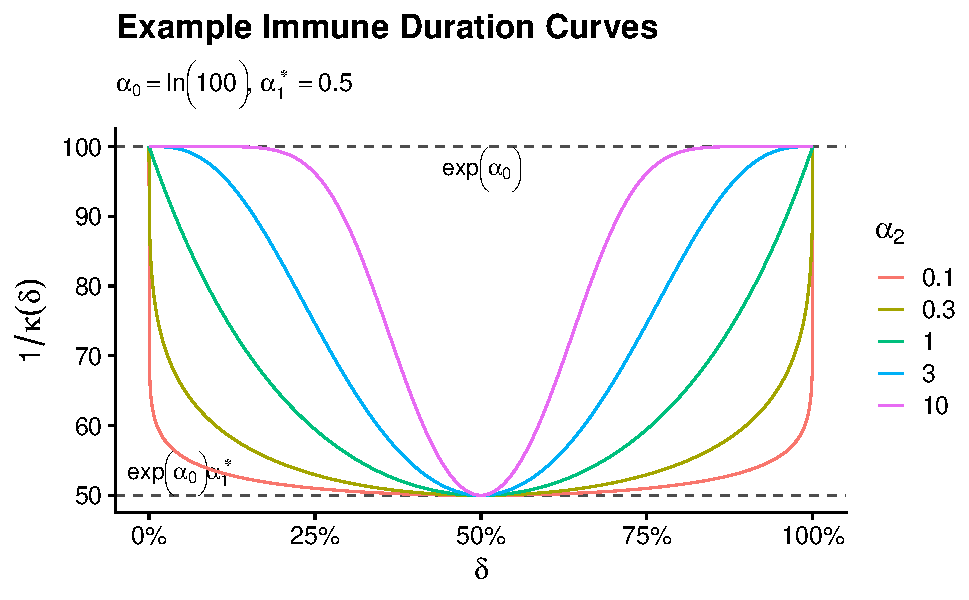
\includegraphics[width=1.0\columnwidth]{example_immune_durration_plot.pdf}
    \caption[Example immune duration curves.]{Example immune duration curves for several values of \( \alpha_2 \), with \( \alpha_0 = \ln\left(100\right), \alpha_1^* = 0.5 \).
    The full formula for these curves is given by \eqref{ch_5:eqn:kappa_delta} and \eqref{ch_5:eqn:alpha_1}.}
    \label{ch_5:fig:example_immune_durration_plot}
\end{figure}

Now, we discuss our model for \( \delta(t) \), the proportion of currently infectious individuals who are infected with the novel variant.
We assume that, after the novel variant is introduced, its proportion in the population evolves according to logistic growth:
\begin{equation}
    \delta(t) = \frac{\exp \left\{ \iota_0 + \iota_1 \left( t \right) \right\}}{\exp \left\{ \iota_0 + \iota_1 \left( t \right) \right\} + 1}.
    \label{ch_5:eqn:logistic_growth}
\end{equation}
To set interpretable priors on \( \iota_0 \) and \( \iota_1 \), we parameterize as 
\begin{equation}
    \delta(t) = \frac{\exp \left\{ \iota_0 + \iota_1 \left( t - t^* \right) \right\}}{\exp \left\{ \iota_0 + \iota_1 \left( t - t^* \right) \right\} + 1}.
\end{equation}
where \( t^* \) is the time point for which \( \delta(t^*) = \frac{ \exp \left\{ \iota_0 \right\} }{\exp \left\{ \iota_0 \right\} + 1} \).
Then \( \iota_1 = \frac{\ln \left( \frac{0.99}{1 - 0.99} \right) - \ln \left( \frac{0.01}{1 - 0.01} \right)}{\iota_1^*} \), where \( \iota_1^* \) is the amount of time the novel variant takes to grow from 1\% of the infectious population to 99\% of the infectious population.

With these parameters all defined, we describe our Bayesian procedure.
We collect all our model parameters into a vector $\boldsymbol{\theta}$ and write the likelihood function as 
\begin{align*}
& \Pr\left(\bW, \bX, \bY, \bZ, \bV^N, \bV^O \mid \btheta \right) \\
=& \Pr\left(\bW \mid \btheta \right) \Pr\left(\bX \mid \btheta \right) \Pr\left(\bY \mid \btheta \right) \Pr\left(\bZ \mid \btheta \right) \Pr\left(\bV^N \mid \btheta \right) \Pr\left(\bV^O \mid \btheta \right)    \\
=&   \prod_{l=1}^{L} \Pr\left(W_l \mid \btheta \right) \Pr\left(X_l \mid \btheta \right) \Pr\left(Y_l \mid \btheta \right) \Pr\left(Z_l \mid \btheta \right) \Pr\left(V^N_l \mid \btheta \right) \Pr\left(V^O_l \mid \btheta \right),
\end{align*}
where \( \Pr\left(W_l \mid \btheta \right) \), \( \Pr\left(X_l \mid \btheta \right) \), \( \Pr\left(Y_l \mid \btheta \right) \), \( \Pr\left(Z_l \mid \btheta \right) \), \( \Pr\left(V^N_l \mid \btheta \right) \), and \( \Pr\left(V^O_l \mid \btheta \right)  \) are the probability mass functions given by \eqref{ch_5:eqn:case_emission}, \eqref{ch_5:eqn:hosp_emission}, \eqref{ch_5:eqn:icu_emission}, \eqref{ch_5:eqn:death_emission}, \eqref{ch_5:eqn:novel_variant_emission}, and \eqref{ch_5:eqn:other_variant_emission}, respectively.
We encode available information about our model parameters in a prior distribution with density $\pi(\btheta)$.
We assume that all univariate non-GMRF distributed parameters are \textit{a priori} independent and list our prior assumptions for our simulation study in Table~tk and for our application in Table~tk.
We base all our inferences and predictions on the posterior distribution of all model parameters:
\begin{equation}
\Pr\left(\btheta \mid \bW, \bX, \bY, \bZ, \bV^N, \bV^O \right) \propto \Pr\left(\bW, \bX, \bY, \bZ, \bV^N, \bV^O \mid \btheta \right) \pi \left( \btheta \right).
\end{equation}
We sample from this posterior using the No-U-Turn Sampler, \citep{NUTS} as implemented in the Turing Julia package \citep{turing}.
Model code and data are available at the following GitHub repository: \url{https://github.com/damonbayer/immunity_semi_parametric_model}.

\section{Results}
\label{ch_5:sec:results}

In our simulation study and application, we observe the non-genetic data at a weekly resolution, while the genetic data is reported at a daily resolution.
We find that the daily reporting of genetic data is crucial to capturing the early exponential-like growth of the novel variant, relative to the other variants.
In addition, to appropriately meet the assumption of logistic growth in \eqref{ch_5:eqn:logistic_growth} we only observe the genetic data after some time, \( t^\dag \), at which we assume the new variant is introduced.
We generally choose \( t^\dag \) to be about one week before the first sequence from the novel variant is observed.

\subsection{Simulation study}
\label{ch_5:subsec:simulation}

We simulate three data sets for this study, each where the novel variant becomes dominant at a different speed: slow (24 weeks to go from 1\% to 99\% of sequences), medium (13 weeks), and fast (7 weeks).
The data sets are simulated from a two strain model, which is depicted in Figure~\ref{ch_5:fig:full_model_diagram_compact} and explained in full detail in Appendix~\ref{ch_5:sec:full_simulation_model_explanation}.
Briefly, the model is similar to the one depicted in Figure~\ref{ch_5:fig:model_diagram} but is modified accounts for two distinct disease variants.
The variants associated with each compartment are indicated by the subscripts: ``N" for the novel variant, ``O" for other variants, and ``A" for all types for variants.
When all compartments associated with one variant type are empty, the model is equivalent to the one from Figure~\ref{ch_5:fig:model_diagram}.

These otherwise independent models are linked by allowing transitions from \( S_B \) and \( R_O \) to \( E_N \).
That is, people who are susceptible to all variant types and those who are only recovered from other variants can become infected with the novel variant.
The rates for these transitions are given by
\begin{equation}
   \lambda_{{S_B}{E_N}}\left( S_B, I_N \right) = \frac{\beta}{N} S_B I_N \quad \textrm{and} \quad \lambda_{{R_O}{E_N}}\left( R_O, I_N \right) = \epsilon \frac{\beta}{N} R_O I_N,
\end{equation}
where \( \beta \) and \( N \) are defined as in \eqref{ch_5:eqn:transition_rates}, and \( \epsilon \in [0, 1] \) is a factor that represents partial immunity to the novel variant conferred by the other variants.
After some time, all the people in the \( O \) subscript compartments will have transitioned to the \( N \) subscript compartments and the model again behaves like the one in Figure~\ref{ch_5:fig:model_diagram}.

\begin{table}
\caption{Simulation parameters that differ by scenario.}
\label{ch_5:table:scenario_differing_parameters}
\centering
\label{table}
\begin{tabular}{lrr}
Scenario & \( \beta \) & \( \epsilon \) \\ \hline
Slow     & 2.1         & 0.75           \\
Medium   & 2.1         & 1.0            \\
Fast     & 3.5         & 1.0            \\
\end{tabular}
\end{table}

\begin{figure}
    \centering
% https://q.uiver.app/?q=WzAsMTMsWzAsMCwiU18wIl0sWzEsMCwiRV8xIl0sWzIsMCwiSV8xIl0sWzIsMSwiUl8xIl0sWzEsMiwiRV97Mn0iXSxbMiwyLCJJXzIiXSxbMiwzLCJSXzIiXSxbMCwyLCJTXzIiXSxbMywwLCJIXzEiXSxbNCwwLCJJQ1VfMSJdLFszLDIsIkhfMiJdLFs0LDIsIklDVV8yIl0sWzQsMSwiRCJdLFswLDFdLFsxLDJdLFsyLDNdLFswLDRdLFs0LDVdLFszLDBdLFszLDRdLFs1LDZdLFs2LDddLFsyLDhdLFs4LDldLFs5LDNdLFs4LDNdLFs1LDEwXSxbMTAsNl0sWzEwLDExXSxbMTEsNl0sWzcsNF0sWzExLDEyXSxbOSwxMl1d
\begin{tikzcd}[sep=scriptsize]
	% {S_0} & {E_1} & {I_1} & {H_1} & {U_1} \\
	% && {R_1} && D \\
	% {S_2} & {E_2} & {I_2} & {H_2} & {U_2} \\
	% && {R_2}
        {S_A} & {E_O} & {I_O} & {H_O} & {U_O} \\
	&& {R_O} && {D_A} \\
	{S_N} & {E_N} & {I_N} & {H_N} & {U_N} \\
	&& {R_N}
	\arrow[from=1-1, to=1-2]
	\arrow[from=1-2, to=1-3]
	\arrow[from=1-3, to=2-3]
	\arrow[from=1-1, to=3-2]
	\arrow[from=3-2, to=3-3]
	\arrow[from=2-3, to=1-1]
	\arrow[from=2-3, to=3-2]
	\arrow[from=3-3, to=4-3]
	\arrow[from=4-3, to=3-1]
	\arrow[from=1-3, to=1-4]
	\arrow[from=1-4, to=1-5]
	\arrow[from=1-5, to=2-3]
	\arrow[from=1-4, to=2-3]
	\arrow[from=3-3, to=3-4]
	\arrow[from=3-4, to=4-3]
	\arrow[from=3-4, to=3-5]
	\arrow[from=3-5, to=4-3]
	\arrow[from=3-1, to=3-2]
	\arrow[from=3-5, to=2-5]
	\arrow[from=1-5, to=2-5]
\end{tikzcd}
    \caption{Caption}
    \label{ch_5:fig:full_model_diagram_compact}
\end{figure}

For our simulations, the compartments are initiated with the entire population (3 million) in \( S_0 \), except a small number who are in \( E_1 \).
Because all the \( N \) subscript compartments are empty, this behaves like the model in Figure~\ref{ch_5:fig:model_diagram}.
We simulate the compartment trajectories until the initial surge begins to subside.
While the overall prevalence is beginning to decrease, we simulate an importation of 1000 people who are infectious with the novel variant into the \( I_2 \) compartment.
Then, the population begins to transition into the \( N \) subscript compartments, resulting in a second wave.
Forecasting this second wave is the objective of our modeling efforts.
We influence the size of this wave and the speed that the novel variant takes over by altering \( \beta \) and \( \epsilon \) in the different simulation settings.
Table~\ref{ch_5:table:scenario_differing_parameters} presents the  the exact \( \beta \) and \( \epsilon \) values used.
The other simulation parameters are given in Table~tk.
The resulting proportion of infectious population with the novel variant over time for each simulated scenario is presented in Figure~\ref{ch_5:fig:proportion_novel_variant_simulated_data_plot}.
The simulated data for the medium takeover speed scenario is plotted in Figure~\ref{ch_5:fig:simulated_binned_data_medium_plot}, with the gray shaded areas indicating the time points for which we create forecasts.
Similar figures for the other data sets are presented in Figures~\ref{ch_5:fig:simulated_binned_data_slow_plot} and \ref{ch_5:fig:simulated_binned_data_fast_plot}.
In each scenario, non-genetic data is reported at a weekly resolution, starting 20 weeks into the simulation, which we call \( t = 0 \).
Genetic data is reported at a daily resolution beginning one week before the novel variant import event.

We fit three models to these simulated data sets: (1) a model where \( R_0(t) \) is a GMRF and \( 1 / \kappa(t) \) constant, (2) a model where \( R_0(t) \) is constant and \( 1 / \kappa(t) \) is a GMRF, and (3) a model where \( R_0(t) \) is constant and \( 1 / \kappa(t) \) is modeled by \eqref{ch_5:eqn:kappa_delta} a function of the proportion of infectious population with novel variant.
The first model is reflective of typical practice in infectious disease modeling.
The second is a slight variation on the first, where we make the immune duration vary over time, rather than the basic reproductive number.
The third model is our main innovation, which models the immune duration based on genetic data.
The priors used in these models are presented in Table~tk.

While these models forecast several data streams, we present only those related to hospitalization in the main text, as this is the most relevant for consumers of these models.
We present results for cases, ICU occupancy, and deaths in Section~\ref{ch_5:sec:sim_cases_icu_death}.
In general, these results exhibit the same patterns as observed in the hospitalization results.
Additionally, we conducted a sensitivity analysis wherein we modified the prior for the anticipated speed of the novel variant takeover and found our model to be robust to these changes.
The results of that analysis are presented in Section~\ref{ch_5:sec:sim_sensitivity}.


\begin{itemize}
    \item x-week ahead forecast plots
    \item CRPS plot
    \item other metrics in appendix
\end{itemize}

\begin{figure}
    \centering
    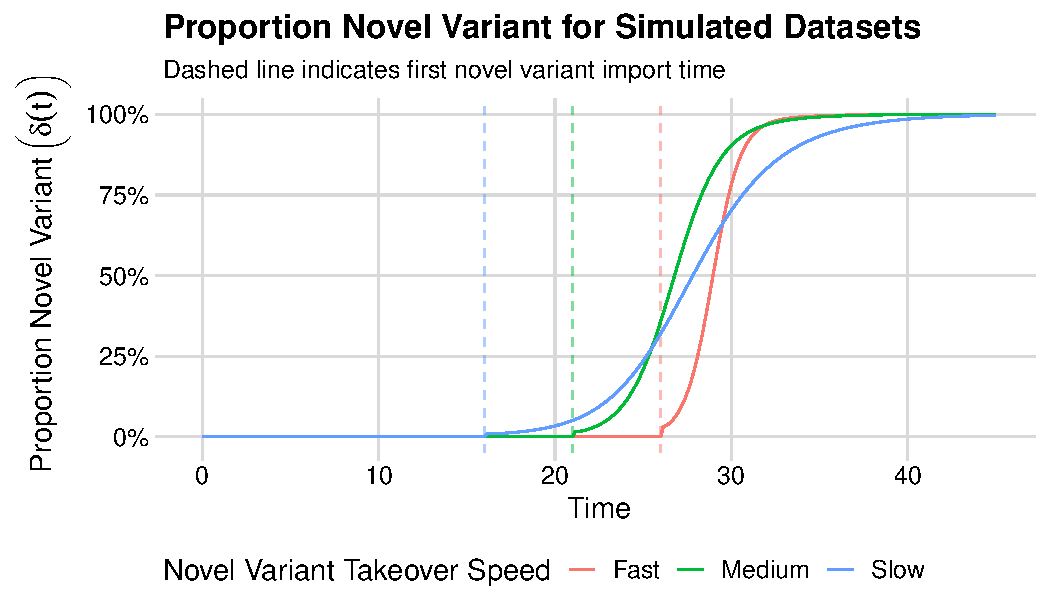
\includegraphics[width=1.0\columnwidth]{proportion_novel_variant_simulated_data_plot}
    \caption{Proportion of infectious population with novel variant over time for three simulated scenarios.
    The dashed line indicates the time that the initial importation event of the novel variant occurs.}
    \label{ch_5:fig:proportion_novel_variant_simulated_data_plot}
\end{figure}

\begin{figure}
    \centering
    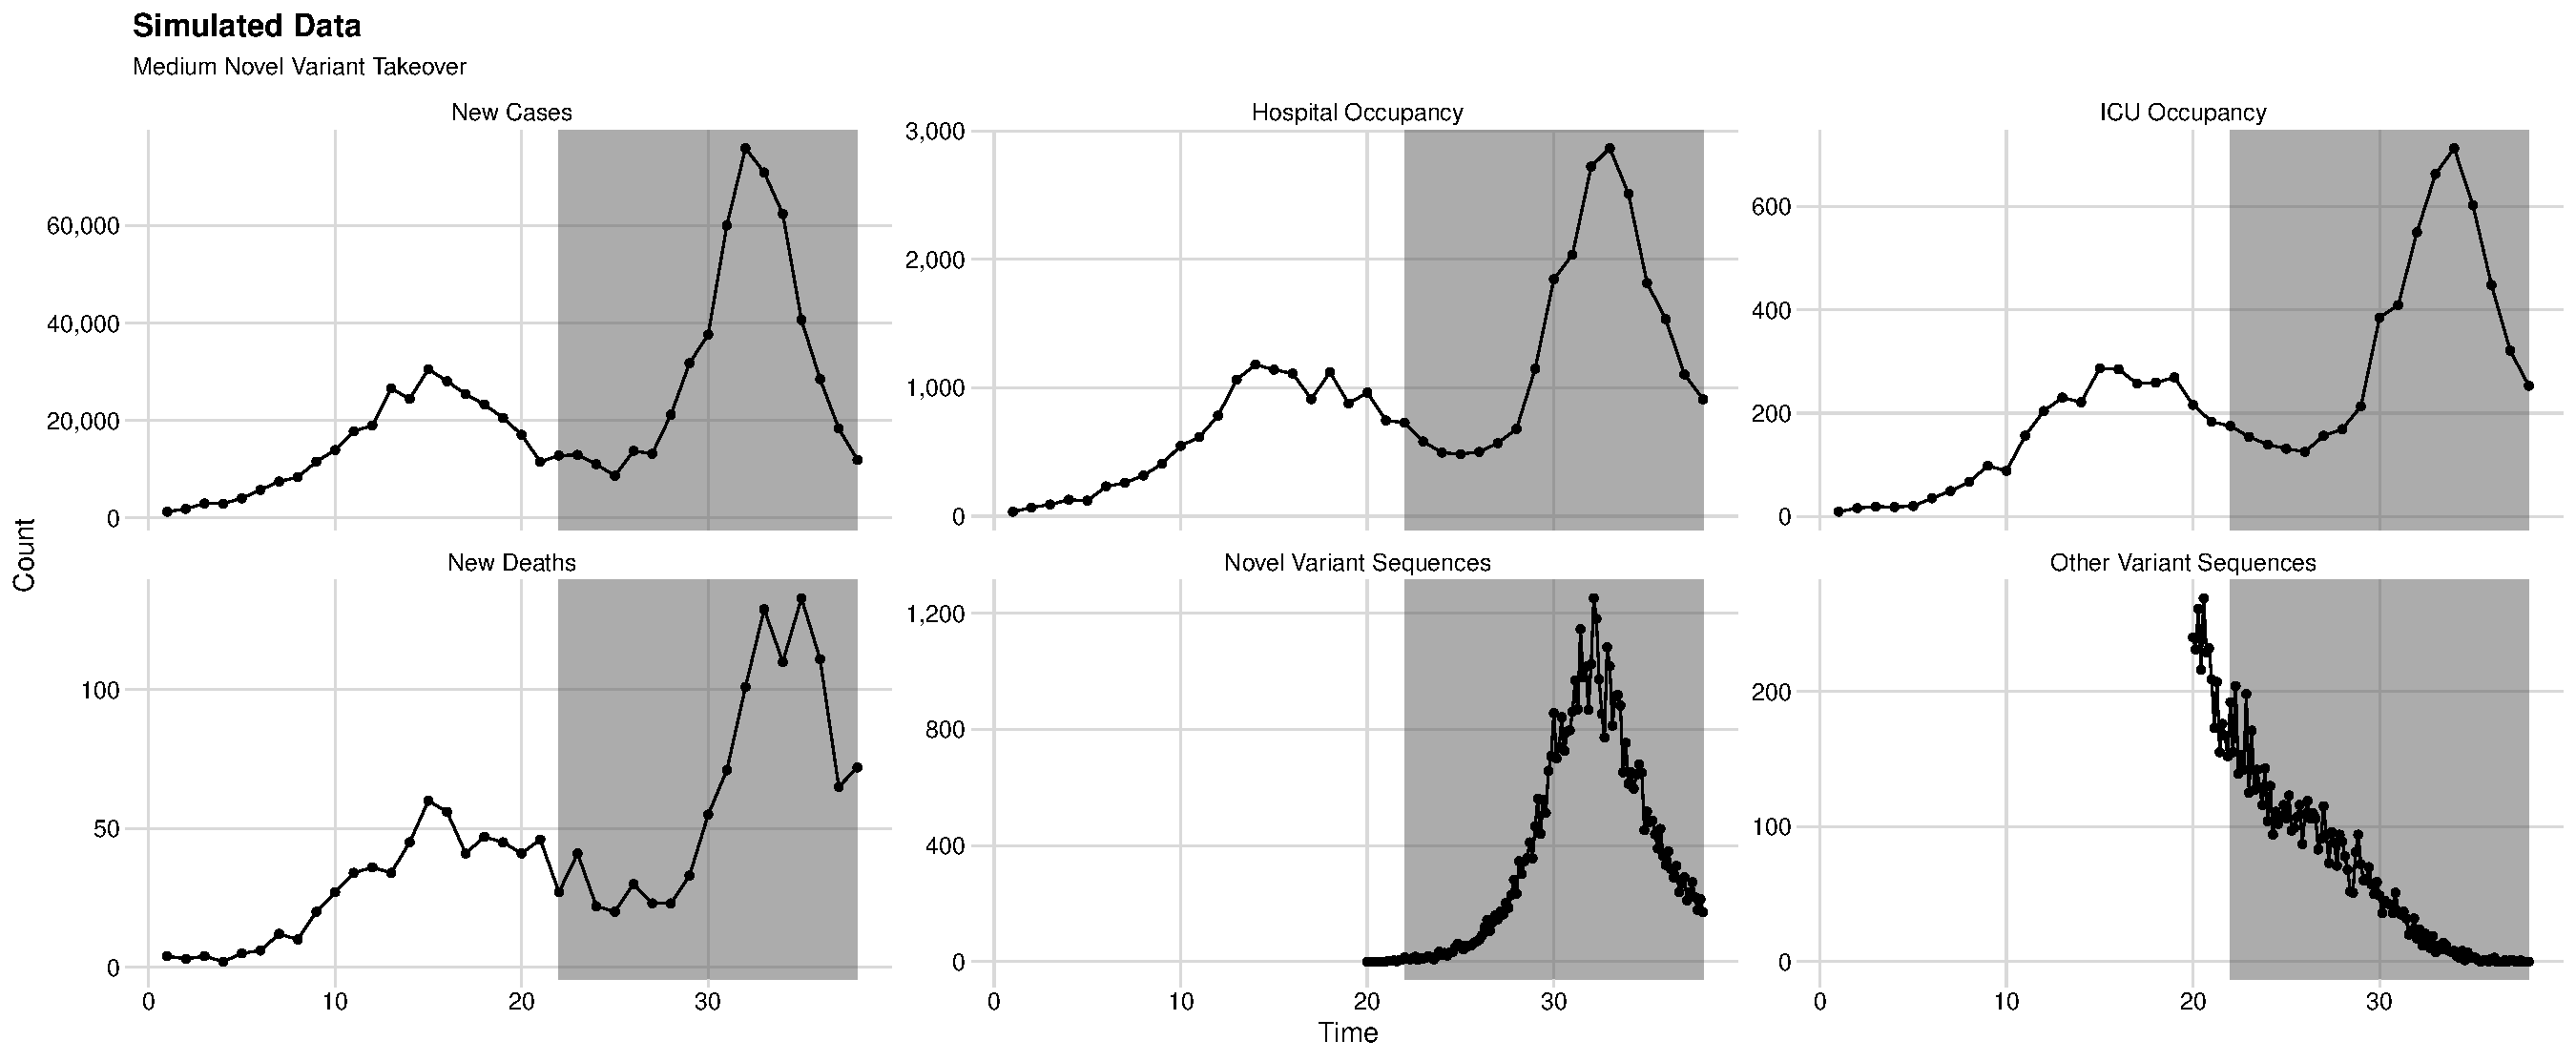
\includegraphics[width=1.0\columnwidth]{simulated_binned_data_medium_plot}
    \caption[Simulated data set for medium takeover speed scenario.]{Simulated data set for medium takeover speed scenario.
    The gray shaded areas indicating the time points for which we create forecasts}
    \label{ch_5:fig:simulated_binned_data_medium_plot}
\end{figure}

In addition, we performed a sensitivity analysis.

\subsection{Application to California data}
\label{ch_5:subsec:application}

In our application, we focus on modeling the wave of cases, hospitalizations, ICU admissions, and deaths associated with the first Omicron variant of SARS-CoV-2 in California.
This wave lasted from roughly December 2021 to March 2022, but we use data beginning in May 2021 to forecast this time period.
We fit models to both Orange County data and statewide data.
The time series of daily counts of positive tests (cases), hospital occupancy and ICU occupancy are provided by the California Department of Public of Health, and published on the California Open Data Portal (\url{https://data.ca.gov}).
Additionally, the daily counts of sequenced viruses, aggregated by pango lineage \citep{pango}, are provided by the Global Initiative on Sharing All Influenza Data (GISAID) \citep{shu2017gisaid} and made available via Outbreak.info \citep{Gangavarapu2023}.
To match the format described in Section~\ref{ch_5:sec:methods}, the lineages are further aggregated into those that begin with ``BA.1" (e.g. BA.1, BA.1.1, BA.1.1.1, BA.1.17.2) and those that do not.
The non-genetic time series are aggregated at a weekly level, while the genetic data is used at a daily resolution.
Figure~\ref{ch_5:fig:california_binned_data_plot} shows the binned data at the statewide level, while Figure~\ref{ch_5:fig:orange_county_binned_data_plot} displays the binned data from Orange County.
The gray highlighted regions indicate the times for which we create forecasts.

\begin{figure}
    \centering
    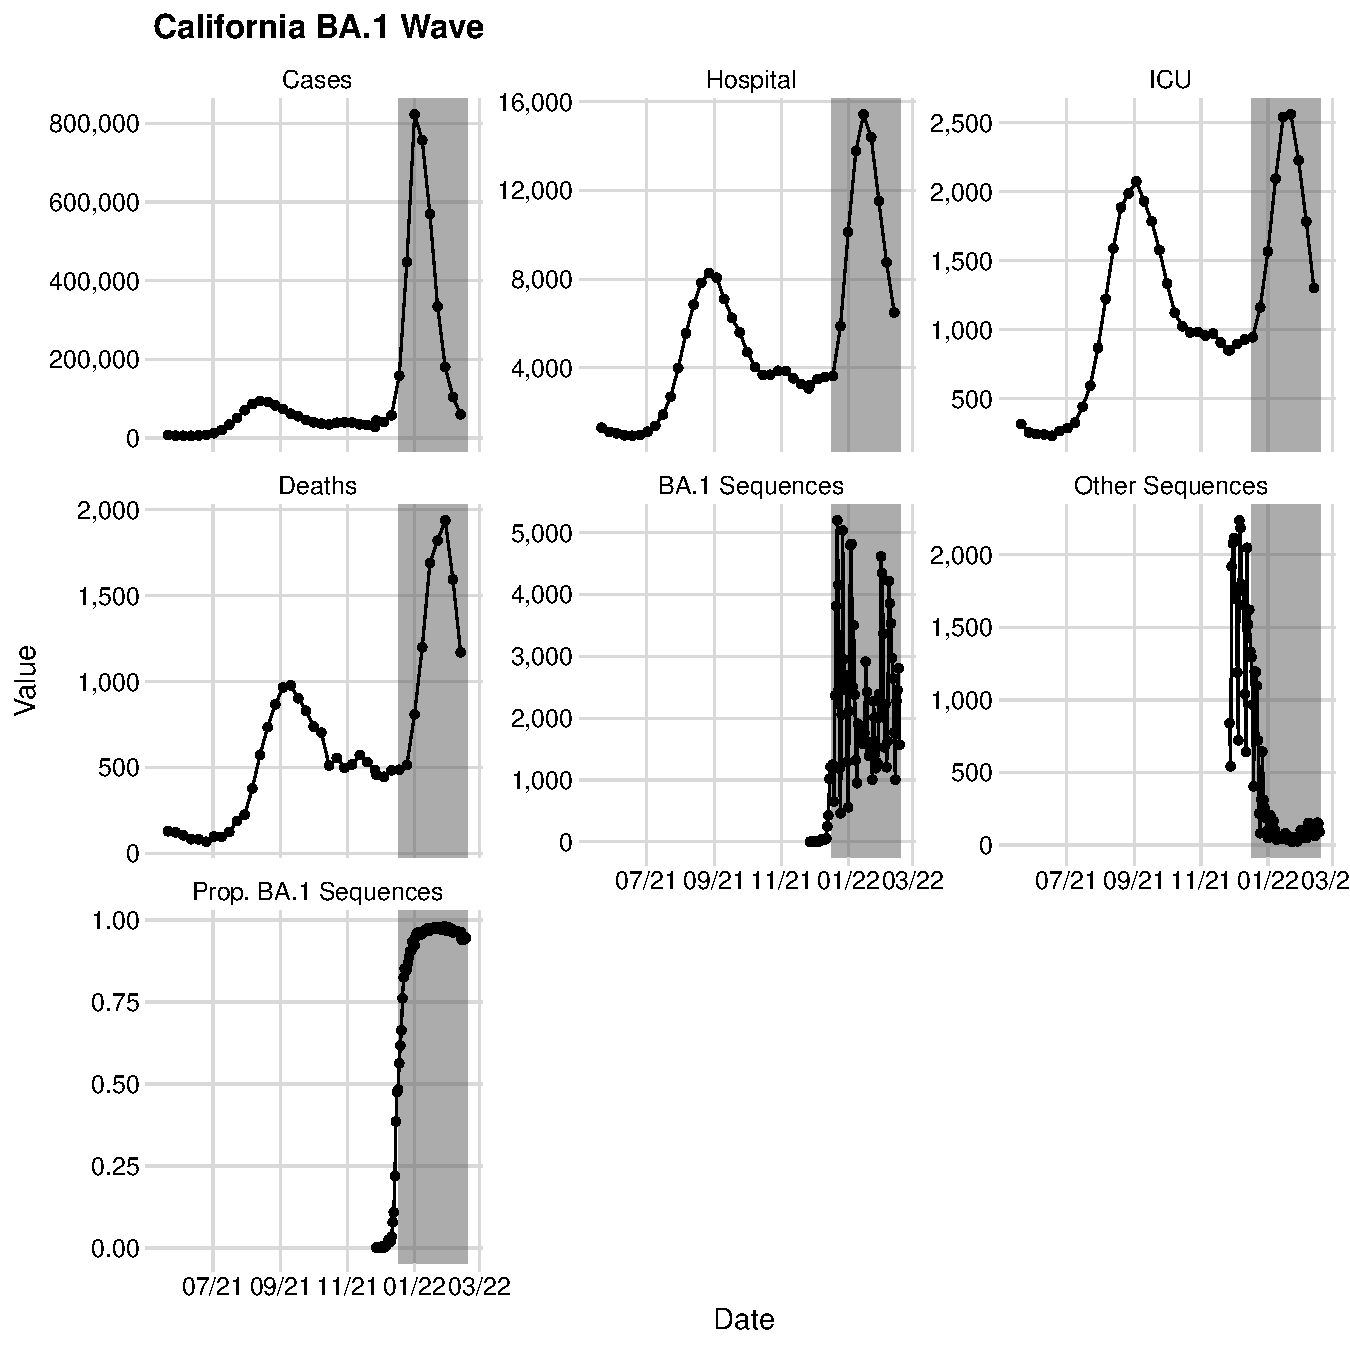
\includegraphics[width=1.0\columnwidth]{california_binned_data_plot.pdf}
    \caption[COVID-19 surveillance data from California.]{
COVID-19 surveillance data from California.
The figure shows weekly counts of cases, hospital and ICU occupancy with OCIVD-19, reported deaths due to COVID-19, as well as genetic virus sequences for BA.1 and non-BA.1 lineages.
The gray highlighted regions indicate the times for which we create forecasts.}
    \label{ch_5:fig:california_binned_data_plot}
\end{figure}

\begin{figure}
    \centering
    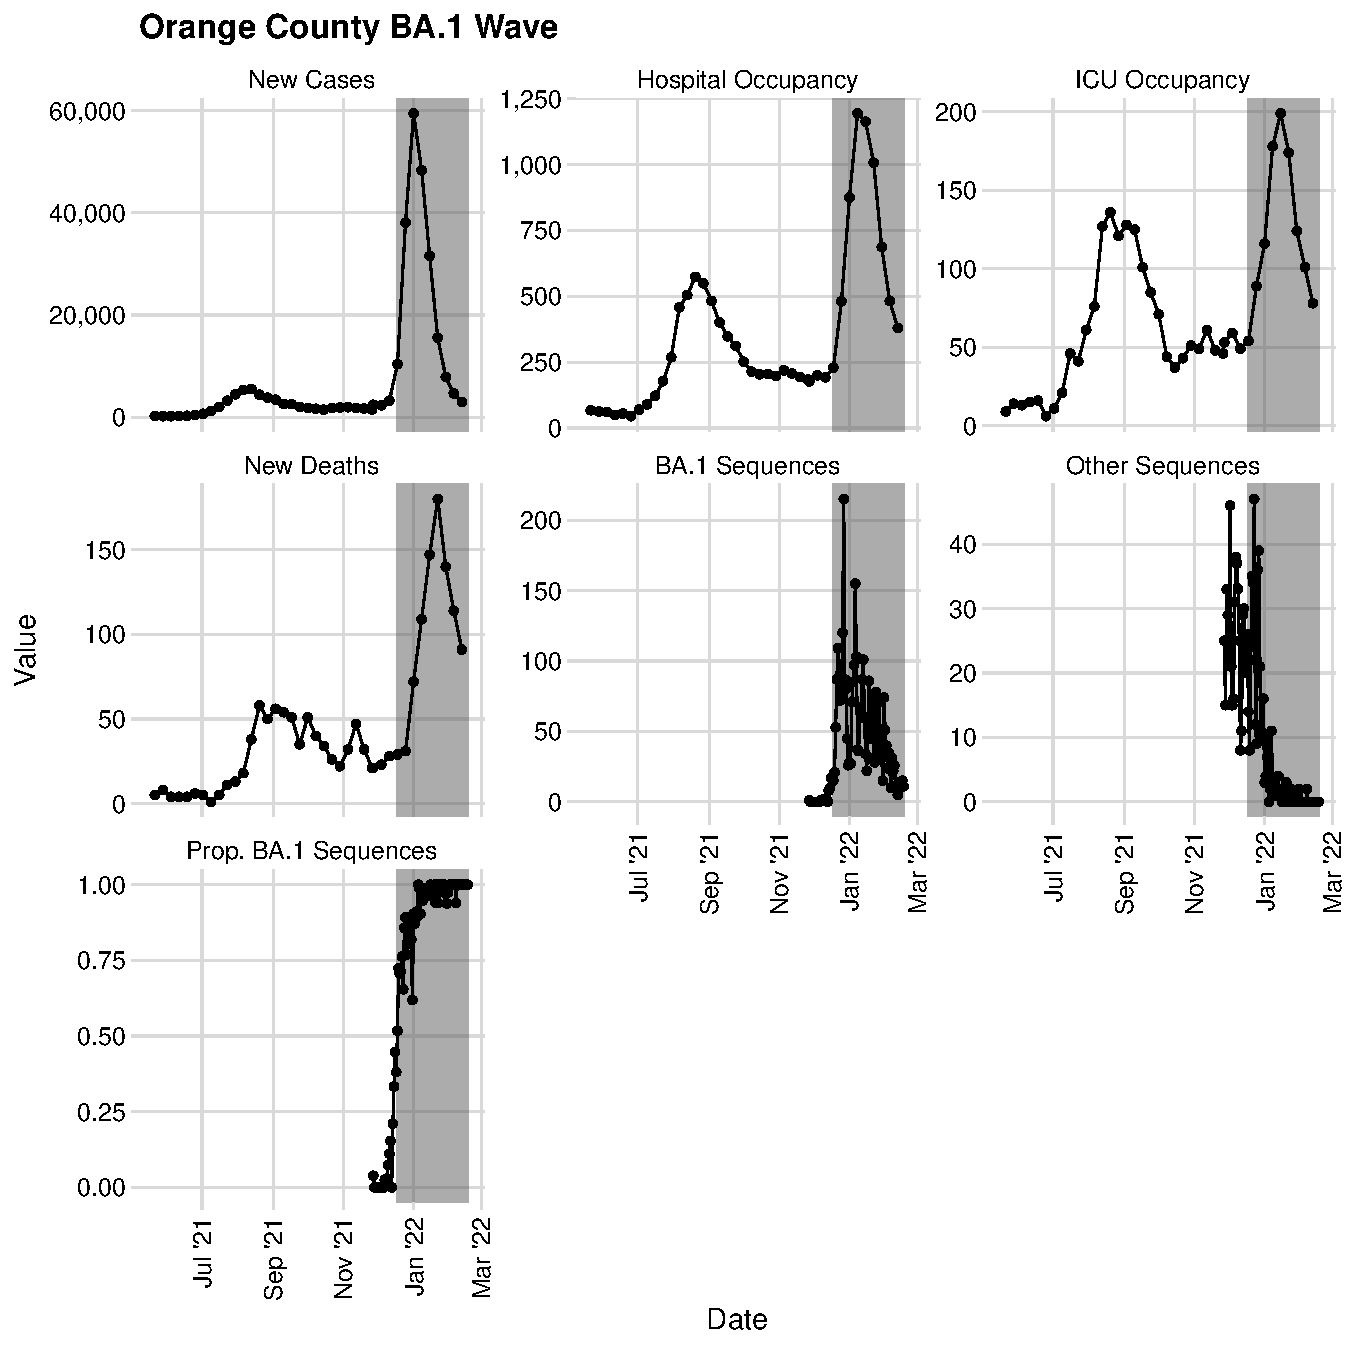
\includegraphics[width=1.0\columnwidth]{orange_county_binned_data_plot.pdf}
    \caption[COVID-19 surveillance data from Orange County, California.]{
COVID-19 surveillance data from Orange County, CA.
The figure shows weekly counts of cases, hospital and ICU occupancy with OCIVD-19, reported deaths due to COVID-19, as well as genetic virus sequences for BA.1 and non-BA.1 lineages.
The gray highlighted regions indicate the times for which we create forecasts.}
    \label{ch_5:fig:orange_county_binned_data_plot}
\end{figure}

\subsection{Discussion}
\label{ch_5:subsec:discussion}
Modeling hospitalization with/for is somewhat complicated.
Assume that with is dominated by for time we care about.
Hospitalization may change for other reasons, but we assume negligible unless there is a natural disaster or something.
We assume that genetic sequences from each variant happens at the same rate, probably not true.
I think there is a note in GISAID or on outbreak.info about this.